%!TEX root = /Users/domaubert/Documents/Lectures/cosmologie/cosmo_main.tex

\chapter{Concepts Fondamentaux}

\section{Définition de l'Univers et de la Cosmologie}
\label{s:fond_def}
 Il faut 3 constituants pour définir complètement un Univers:
\begin{enumerate}
\item un contenu en énergie, qui peut être sous diverses formes,
\item un jeu de lois physiques qui régissent l'entrejeu des différentes énergies,
\item un espace-temps\index{espace-temps}, qui est la scène sur laquelle cet entrejeu prend place.
\end{enumerate} 
L'enjeu de la \textit{cosmologie} est précisément d'étudier le contenu, les lois physiques et la structure de l'Univers. Par conséquent la cosmologie est liée aux aspects théoriques les plus fondamentaux de la physique mais également à des problèmes astrophysiques et il existe plusieurs manières de faire de la cosmologie. On cherchera par exemple à déterminer quelles sont les lois à l'œuvre dans le cosmos (point 2) , ce qui est davantage du domaine de la physique théorique, ou bien à déterminer les paramètres (point 3)  qui caractérisent la structure spatio-temporelle (e.g. sa forme ou bien son histoire) de l'Univers comme en cosmologie observationnelle. De même comprendre comment les différentes formes d'énergie (matière, lumière, etc...) s'organisent ou évoluent au cours du temps (point 1) (e.g. comment les grandes structures de l'Univers se mettent en place) permet d'avoir un éclairage sur les deux autres aspects du problème cosmologique.

\section{Principe Cosmologique}\index{principe cosmologique}
L'objectif de la cosmologie est ambitieux et cette ambition n'est pas sans obstacles. L'un des problèmes les plus importants est notre incapacité à garantir que ce que nous observons autour de nous reste valable à l'échelle du cosmos, \textit{y compris dans les régions de l'Univers qui nous serons à jamais inaccessibles}. Par exemple, rien ne garantit absolument que la neutralité électrique\index{neutralité électrique} soit vraie dans tout le cosmos ou bien que la densité de matière mesurée dans notre Univers observable soit effectivement celle de l'Univers entier\sidenote{on distingue parfois \textit{Cosmos} et \textit{Univers}, où le Cosmos est la sous-partie de l'Univers qui nous est accessible. Par simplicité, aucune différence ne sera faite entre les deux termes dans cet ouvrage.}. Aujourd'hui, il ne viendrait à l'idée de personne d'attribuer au cosmos une densité égale à celle de la Terre, pour autant c'est peu ou prou ce que nous faisons en cosmologie. 

Pour autant, \textit{nous n'avons pas le choix}. Par définition, il est impossible de connaître les propriétés de régions dont on ne peut extraire de l'information et toujours par définition, il existe de telles régions dans l'Univers. Quelle option reste-t-il à la personne désireuse de faire de la science à l'échelle de l'Univers, si ce n'est de supposer que ce qui nous est accessible est valide dans tout le cosmos ? Aucune : en l'absence d'une telle hypothèse, il est tout simplement impossible de faire de la science avec l'Univers.

Cette supposition est à la base du \textit{Principe Cosmologique}\index{principe cosmologique}. Si nous revenons sur les 3 constituants définis en début de chapitre, il est aisé de reconnaître que cette supposition implique que le contenu universel en énergie doit être le même que celui que nous constatons autour de nous. De même, la structure spatio-temporelle universelle doit être la même que celle que nous constatons dans l'Univers observable. Toutefois cette hypothèse "universaliste" implique également que nous supposons que les même lois de la nature s'appliquent dans tout le cosmos, y compris dans les régions qui nous sont inaccessibles ou pour lesquelles l'information n'est pas extractible. Le \textit{Principe Cosmologique} que nous retiendrons est le suivant : le contenu en énergie de l'Univers, sa structure spatio-temporelle et les lois qui y opèrent sont les même partout et par conséquent sont celles que nous constatons autour de nous. Notons tout de suite que cette universalité des composants s'applique aux échelles pertinentes pour la cosmologie et n'empêche pas des départs locaux aux valeurs universelles.

\subsection{Tautologie}

A ce stade, il nous semble que la cosmologie peut être définie par une tautologie~: \textit{la cosmologie est la science qui met le principe cosmologique à l'épreuve.} Si nous nous retrouvons dans une situation qui reste inexplicable dans ce que nous croyons être le jeu universel de contenu énergétique, spatio-temporel et "législatif" de l'Univers, alors les options sont réduites:
\begin{itemize}
\item soit nous continuons de croire que le principe cosmologique reste valide et c'est le détail de son contenu qui doit être révisé. Par exemple on modifiant les lois de la physique pour qu'elles rendent compte des nouveaux phénomènes tout en continuant à être une bonne description des processus locaux. C'est la voie scientifique standard.
\item soit nous renonçons au principe cosmologique et donc à l'universalité de ses composants et nous renonçons en même temps à l'ambition de décrire tout l'Univers avec la science que nous connaissons.
\end{itemize}

\subsection{Principe cosmologique pragmatique}
Le principe cosmologique est souvent décliné dans une version plus pragmatique qui est la suivante:
\begin{enumerate}
\item la gravitation est correctement décrite par la théorie de la relativité générale d'Einstein \index{relativité générale},
\item l'Univers est homogène et isotrope\index{homogénéité}\index{isotropie}.
\end{enumerate}
Le point 2 revient à appliquer au cosmos ce que nous voyons de l'état de l'Univers autour de nous (contenu, géométrie, évolution etc...). Le point 1 revient à définir les lois universelles de la gravité~: une emphase particulière est mise sur cette interaction\sidenote{On rappelle qu'on distingue 4 interactions fondamentales \index{interaction fondamentale} : la \textit{gravitation}, la \textit{force électromagnétique} et les deux forces corpusculaires\textit{ fortes} et \textit{faibles}.} car elle est la seule qui \textit{in fine} est toujours de portée infinie et donc cosmologique. Par ailleurs, une fois la théorie de relativité générale\index{relativité générale} choisie comme description correcte de la gravité, le point 2 a des conséquences sur les régimes qui vont être explorés avec cette théorie.

\section{Relativité Générale: notions}
La gravitation\index{gravitation} est centrale à l'étude de la cosmologie car elle est la seule "force"\index{force} dont l'action ne peut être écrantée et dont la portée soit infinie \sidenote{les forces corpusculaires sont de courte portée tandis que la force électromagnétique est en pratique toujours écrantée car une charge n'est jamais isolée de charges opposées sur les échelles qui nous intéressent}. De fait, elle est la seule force qui soit effective lorsque des échelles cosmologiques sont abordées. De plus la gravitation peut être décrite comme la manifestation des propriétés de l'espace-temps. Or il s'avère que la structure spatio-temporelle de l'Univers n'est pas triviale comme l'indique par exemple le phénomène d'expansion de l'Univers. Par conséquent l'observation de l'expansion du cosmos nous dit également des choses sur la façon dont la gravitation est à l'œuvre dans le cosmos. Compte tenu du rôle central de la gravitation pour les études cosmologiques, nous allons faire un aperçu de la théorie de la relativité générale\index{relativité générale} et sur son application dans le cadre cosmologique\sidenote{le lecteur intéressé pourra par exemple se reporter à l'excellent ouvrage d'introduction \textit{A first course in general relativity} par B. Schutz.}.

\subsection{Principe d'équivalence}
Le principe d'équivalence\index{principe d'équivalence} existe sous forme de différentes saveurs. La plus triviale est la suivante, où l'on considère le principe fondamental de la dynamique :
\begin{equation}
\frac{F_z}{m_i}=\ddot z.
\end{equation}
Ici l'on explique que l'accélération\index{accélération} suivant la direction z est \textit{proportionnelle} à la force appliquée au système étudié et \textit{inversement proportionnelle} à un coefficient, que l'on nomme \textit{masse inertielle}\index{masse inertielle}. Par conséquent, deux systèmes soumis à la même force vont réagir différemment selon les valeurs du coefficient $m_i$ qui les caractérisent. Intuitivement on comprend assez rapidement que ce coefficient est lié à la quantité de matière que le système possède, d'où son qualificatif de masse~: soumis à la même force, un système fortement chargé en matière réagira moins qu'un système ayant une quantité de matière plus faible. Maintenant considérons l'expression de $F_z$ si cette force se trouve être une force de pesanteur \sidenote{c'est à dire le poids}:
\begin{equation}
F_z=m_g g
\end{equation}
où g est la norme du champ de pesanteur. Cette force $F_z$ est d'autant plus forte que le coefficient $m_g$ est important~: ce coefficient caractérise également la quantité de matière dans le système et un système avec une grande quantité de masse va naturellement avoir une valeur élevée de $m_g$ et donc une pesanteur importante. Cette masse $m_g$ est aussi dénommée \textit{masse grave}\index{masse grave}.

A ce stade, nous avons donc deux coefficients qui tracent la quantité de matière dans un système physique:le premier $m_i$ lié aux équations de la dynamique, et sans aucune référence à priori à une force de pesanteur (ou de gravitation),  et le second $m_g$ qui lui pour le coup est complètement lié à la présence d'un champ de pesanteur. Il faut alors se rappeler qu'à priori, \textit{rien} ne nous informe d'une quelconque relation quantitative entre les deux et qu'il faut postuler une éventuelle relation entre les masses inertielles et graves.

Toutefois, l'expérience nous indique que tous les systèmes soumis à un champ de pesanteur donné semblent posséder la même accélération $\ddot z$ et ceci quelles que soient leurs masses inertielles et graves. Ceci implique que $m_g\sim m_i$. Plutôt qu'une vague égalité, \textit{le principe d'équivalence} stipule une exacte identité entre ces deux quantités:
\begin{equation}
m_g=m_i.
\end{equation}
Cette égalité est fortement suggérée par l'expérience, mais ne peut être démontrée comme étant absolument valide \sidenote{actuellement les mesures expérimentales excluent toute différence relative entre les 2 masses supérieure à $10^{-12}$}. Selon ce principe, la quantité de matière intervient au travers d'une valeur unique qui est \textit{la masse} $m=m_g=m_i$. On peut noter dès à présent que cette égalité confère à la gravitation un rôle spécial~: la masse \textit{inertielle} est liée à la loi décrivant la dynamique des systèmes, y compris en l'absence de gravitation. Par exemple, une particule chargée dans un champ électrique verra son accélération modulée en $q/m_i$. La force électrostatique, comme toutes les autres forces subit l'impact de ce coefficient d'origine dynamique. D'après le principe d'équivalence\index{principe d'équivalence}, la gravitation quant à elle possède \textit{dans sa propre expression} ce même coefficient, avant expression d'un quelconque problème dynamique. Elle dispose donc de façon innée d'une sorte d'élément d'information sur la façon dont la dynamique est régie, information que ne possèdent pas les autres interactions.

\subsection{Référentiel inertiel}
L'équivalence entre masse grave et inertielle a plusieurs conséquences. Comme déjà mentionné, elle permet de rendre compte de l'universalité de l'accélération de systèmes différents dans un même champ de pesanteur. C'est la fameuse expérience de la tour de Pise où des masses différentes lâchées de la même hauteur parviennent au sol au même instant car étant accélérées exactement de la même façon. Il en découle également que si l'on fait le choix d'étudier la chute libre\index{chute libre} de plusieurs objets dans un référentiel lui même en chute libre, ces objets apparaissent tous comme en "flottaison" comme si l'on avait annulé la gravitation dans ce référentiel\index{référentiel} et ceci même si ils sont tous très différents. A nouveau cela n'est possible que parce que la chute libre dans un champ de pesanteur est la même quel que soit l'objet considéré. 

\begin{figure}[htbp]
	\centering
		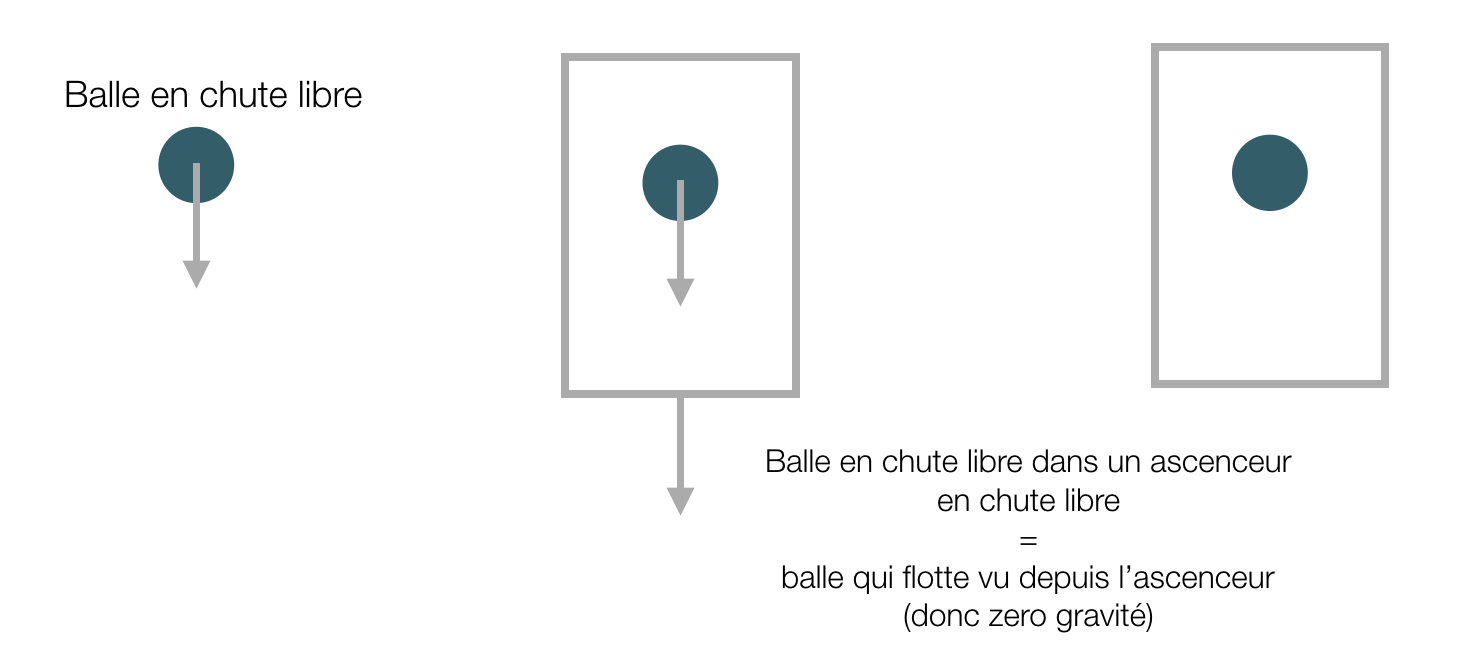
\includegraphics[height=10cm]{figs/ascenceur.png}
	\caption[Annulation du champ de pesanteur]{Dans cette expérience de pensée, on considère une balle en chute libre dans un champ de pesanteur. Si on encage cette balle dans un ascenceur lui-même en chute libre, on crée un référentiel concrétisé par les parois de l'ascenseur, à l'intérieur duquel la balle 'flotte'. Dans ce jeu de coordonnées précis, on annule la gravitation : un observateur à l'intérieur de l'ascenseur est incapable de dire si on a éteint la gravité, ou bien si il se trouve dans un ascenceur en chute libre. Notons que comme tous les objets tombent à la même vitesse, l'observateur ne peut pas se renseigner en faisant la même expérience avec des objets divers : tous les objets, quelles que soient leurs masses et leurs compositions vont flotter de la même manière. }
	\label{f:ascenceur}
\end{figure}


Ce type de référentiel est appelé \textit{référentiel inertiel}\index{référentiel inertiel}. Généralement un tel référentiel ne peut être construit que localement et par exemple dans un champ de pesanteur radial, il est possible de construire une collection de référentiel inertiels qui annuleront la gravité localement mais aucun de ces référentiels ne peut annuler globalement le champ de pesanteur. A ce titre il est usuel de se référer à ce type de référentiel sous l'appellation \textit{référentiel localement inertiel}. Cette possibilité d'annuler localement la gravité est intrinsèquement lié à l'égalité $m_i=m_g$. Ce lien est si fort que l'on va considérer que \textit{la possibilité d'annuler la gravitation par un choix approprié de référentiel local est aussi un énoncé du principe d'équivalence}. 

\begin{figure}[htbp]
	\centering
		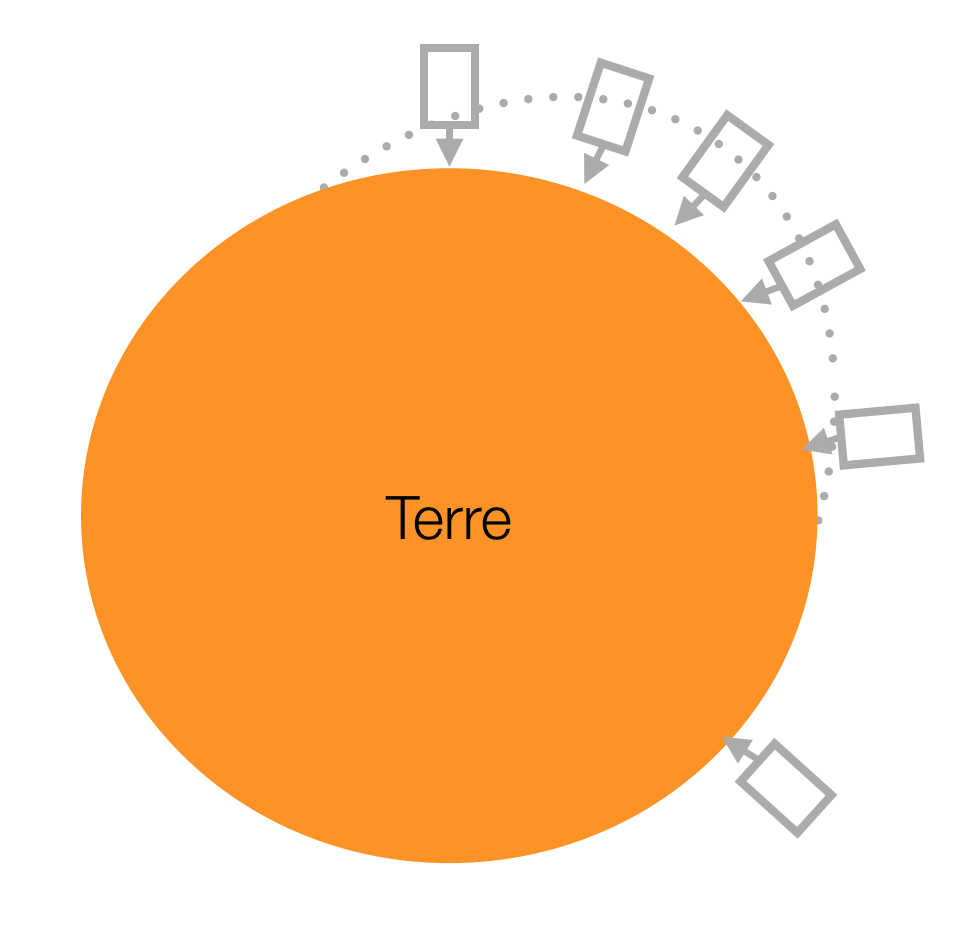
\includegraphics[height=10cm]{figs/ascradial.png}
	\caption[Référentiels localement inertiels]{Tous ces ascenseurs en chute libre, \textit{localement}, vont annuler le champ de pesanteur. En revanche, ils sont tous orientés différemment, suivant le champ de pesanteur local : on ne peut pas construire un système de référence global qui annule tous les champs de gravité. Ces référentiels inertiels sont locaux.}
	\label{f:ascradial}
\end{figure}

De fait, cette approche renverse le point de vue habituellement adopté sur le comportement mécanique des objets. Le point de vue newtonien classique consiste à supposer l'existence d'un champ de pesanteur qui va par exemple 'tordre' la trajectoire d'un objet initialement rectiligne en une parabole \sidenote{c'est le cas par exemple de la trajectoire balistique standard en $z(t)=-\frac{g t^2}{2}+V_0 t +x_0$.}. Dans l'approche relativiste, la trajectoire d'un système est toujours rectiligne dans les référentiels localement inertiels : en effet, en l'absence de pesanteur, le système se déplace toujours en ligne droite. Mais comme les référentiels ne sont pas tous 'alignés' les uns avec les autres, la trajectoire apparaît comme 'tordue' : les systèmes se propagent en ligne droite dans des systèmes de références qui ne sont pas 'alignés', créant ainsi toutes les variétés de trajectoires que nous connaissons. 


Notez qu'à l'aide d'un choix approprié de référentiel on peut également créer de la gravité. Si des systèmes libres sont placés dans un référentiel uniformément accéléré, ils percevront leur mouvement relatif comme induit par une force de gravitation. \textit{De façon générale il est impossible localement de distinguer un référentiel uniformément accéléré d'un champ de gravitation.}


\subsection{Qu'est-ce que la gravitation ?}
A nouveau, on peut créer ou "détruire" un champ gravitationnel par un choix approprié de référentiel. Or un référentiel pourrait se résumer à un ensemble de règles étalons et d'horloges ayant un certain comportement donc à un objet qui n'a qu'une nature géométrique et non pas physique. A partir de cette constatation, il est tentant de considérer alors que la gravitation n'est qu'une manifestation géométrique de l'espace dans lequel évoluent les systèmes. C'est le choix que fait la théorie de la relativité générale\index{relativité générale} (RG par la suite), où la gravitation n'est pas une force à proprement parler mais davantage une manifestation de la géométrie\index{géométrie} de l'espace-temps\index{espace-temps}. En RG, les systèmes se déplacent librement dans une géométrie qui, si elle est non triviale, produit des effets qui peuvent être interprétés comme le produit d'une interaction. A ce titre on peut dire que \textit{la gravitation n'existe pas}, elle n'est qu'une interprétation d'un effet de nature fondamentalement géométrique. 

Ainsi, on verra par la suite que c'est la courbure de cette géométrie qui produit les effets gravitationnels \sidenote{mathématiquement, cela se manifeste par des dérivées secondes de la géométrie par rapport aux variables qui décrivent l'espace-temps}. A l'inverse, une géométrie sans courbure\index{courbure}, i.e. une géométrie plane, produit un environnement sans effets de gravitation. Or il est aisé d'imaginer qu'il est toujours possible de trouver \textit{localement} un jeu de coordonnées qui rendent une géométrie plane, i.e. une transformation \textit{locale} qui permette de détruire la gravitation. Par analogie, une fonction régulière peut être approximée comme une collection de tangentes sur lesquelles il n'y a pas de courbures et qui localement sont des représentations exactes de la fonction originale. C'est une manifestation du principe d'équivalence~:\textit{il est toujours possible de trouver une transformation locale qui rende la géométrie de l'espace-temps plane}. Plus précisément c'est parce que l'on considère la gravitation comme étant de la géométrie que le principe d'équivalence se trouve naturellement réalisé.

Cette capacité à créer un jeu de coordonnées qui puisse annuler la gravitation est d'une importance majeure, pour la physique en général. En effet, comment faire pour faire de la physique en présence d'un champ de gravitation ? Il suffit d'annuler la gravitation, par un choix approprié de système de référence, pour retomber sur le cas sans gravitation et que généralement on arrive à formuler. D'un point de vue technique, si l'on parvient en l'absence de gravitation à exprimer les lois dans la nature dans une formulation qui s'accommode de changements de référentiels 'propres' \sidenote{on parle de formulation \textit{covariante}}, nous sommes capables de les exprimer en présence de gravitation car il existe toujours un 'point de vue' qui permet d'annuler ses effets. C'est le cas par exemple des lois de l'électromagnétisme, qui possèdent une telle formulation.

Cette vue de la gravité comme géométrie de l'espace-temps est l'école classique d'interprétation de la RG. Elle n'est toutefois pas sans poser problème par exemple si l'on cherche à quantifier la gravitation\index{gravitation quantique}. Si cette dernière est pure géométrie alors on peut arguer qu'il n'y a rien à quantifier et par exemple il n'y a pas de raison à priori d'invoquer l'existence d'un boson\index{boson} porteur de l'interaction, coupant court à toute tentative de quantification et donc d'unification. Si l'on estime que la quantification\index{quantification} est nécessaire alors la vision géométrique n'est qu'une interprétation, certes très puissante, d'un processus qui n'est pas pure géométrie. Dans ce cadre le principe d'équivalence devient prééminent: il faut le supposer réalisé par un mécanisme encore inconnu et sa réalisation conduit à une possible interprétation géométrique \sidenote{c'est par exemple l'approche adopté par S. Weinberg dans le livre \textit{Gravitation \& Cosmology} }. L'approche classique vue précédemment raisonne de façon inverse.

\subsection{Espace-temps et Métrique}
La théorie de la relativité générale décrit la gravitation comme une manifestation de la géométrie de l'espace-temps\index{espace-temps}. Cet espace temps possède 4 dimensions, une de temps et trois d'espace. L'outil mathématique permettant de décrire cette géométrie est la géométrie différentielle\index{géométrie différentielle}. Une quantité centrale est \textit{la métrique}\index{métrique}~: fondamentalement elle est l'outil qui permet de calculer des distances (des produits scalaires) dans une géométrie arbitraire. En notation d'Einstein\index{notation d'Einstein}\sidenote{la notation d'Einstein consiste à omettre le signe de sommation sur les indices répétés. Par exemple $g_{\alpha\beta} x^\alpha =\sum_\alpha g_{\alpha\beta} x^\alpha$ }, le calcul d'une distance\index{distance} s'écrit de la façon suivante :
\begin{equation}
ds^2=g_{\mu\nu}dx^\mu dx^\nu,
\label{e:scal}
\end{equation}
où les indices $\mu,\nu$ courent sur les indices des coordonnées, $ds^2$ est un scalaire donnant la distance couverte par un intervalle\index{intervalle} $(dx^0,dx^1,dx^2,dx^3)$. La quantité $g_{\mu\nu}$ est la métrique et permet de relier la distance aux composantes de l'intervalle\index{intervalle}. Si la géométrie est plane, la métrique aura une certaine forme et si la géométrie est courbe et complexe, cette expression sera différente. En géométrie euclidienne\index{géométrie!euclidienne} plane à 3D le calcul de distance est le suivant:
\begin{equation}
ds^2=(dx^1)^2+(dx^2)^2+(dx^3)^2.
\end{equation} 
En géométrie de Minkowski\index{géométrie!Minkowski}, correspondant à l'espace-temps plat utilisé par la relativité restreinte, le calcul devient
\begin{equation}
ds^2=(dx^0)^2 -((dx^1)^2+(dx^2)^2+(dx^3)^2)
\end{equation} 
où $dx^0=cdt$ est la composante liée au temps. L'expression générale est elle donnée par Eq. \ref{e:scal}.

Cette métrique synthétise la structure spatio-temporelle de la \textit{variété} que l'on cherche à étudier. Pour faire de la cosmologie, il faut ainsi se doter d'une telle métrique, la plus à même de représenter ce que l'on croit être les caractéristiques génériques du cosmos.

\subsection{Métrique de Friedmann-Robertson-Walker}
En se rappelant l'énoncé du principe cosmologique\index{principe cosmologique} pragmatique, la métrique devant servir à décrire l'Univers doit refléter les propriétés d'homogénéité et d'isotropie\index{homogénéité}\index{isotropie}. La métrique la plus générique satisfaisant ces contraintes est la métrique de Friedmann-Robertson-Walker (FRW)\index{Friedmann-Robertson-Walker!métrique}. A l'aide de celle-ci, l'intervalle de distance 4D est donné par:
\begin{equation}
ds^2=c^2dt^2-a(t)^2(\frac{dr_0^2}{1-Kr_0^2}+r_0^2d\theta^2+r_0^2\sin^2\theta d\phi^2).
\label{e:FRW}
\end{equation}
On note que cette métrique fait usage d'un système de coordonnées sphériques $(r_0,\theta,\phi)$ pour sa partie espace. On note également que par rapport aux exemples Euclidien et Minkowskien, FRW couple explicitement les parties temporelles et spatiales, via le facteur d'expansion \index{facteur d'échelle} $a(t)$ \sidenote{appelé aussi facteur d'échelle}.  

$r_0$ est une \textit{distance comobile}\index{distance!comobile}~: c'est une coordonnée de nature spatiale et indépendante du temps. Ici elle désigne une distance radiale prise à partir de l'origine du système de coordonnées et est également prise en compte pour calculer les contributions à l'intervalle des séparations angulaires $d\theta$ et $d\phi$. Le paramètre $K$ est un paramètre \textit{de courbure} auquel on peut éventuellement associer un rayon de courbure\index{courbure} $R_K=K^{-1/2}$ \sidenote{une simple analyse dimensionnelle montre par exemple que $Kr_0^2$ doit être sans dimension}.

Si l'on considère deux évènements sur une même ligne de visée\index{ligne de visée} (donc avec $d\theta=d\phi=0$), l'intervalle peut se représenter sous une forme
\begin{equation}
ds^2=c^2dt^2-dr^2,
\end{equation}
avec 
\begin{equation}
dr=\frac{a(t)dr_0}{\sqrt{1-Kr_0^2}}.
\label{e:phydist}
\end{equation}
Ici $dr$ désigne la distance \textit{physique}\index{distance!physique} de la partie spatiale (donc 3D) de l'intervalle que nous étudions. Cette distance dépend du temps, donc de l'instant considéré, et est modulé par une éventuelle courbure. A proximité de l'origine ($r_0\rightarrow 0$) ou dans des régimes de très faible courbure ($R_K\rightarrow\infty$ ou $K\rightarrow 0$), distance physique et distance comobile sont directement reliées par :
\begin{equation}
dr=a(t)dr_0.
\end{equation}

\begin{figure}[htbp]
	\centering
		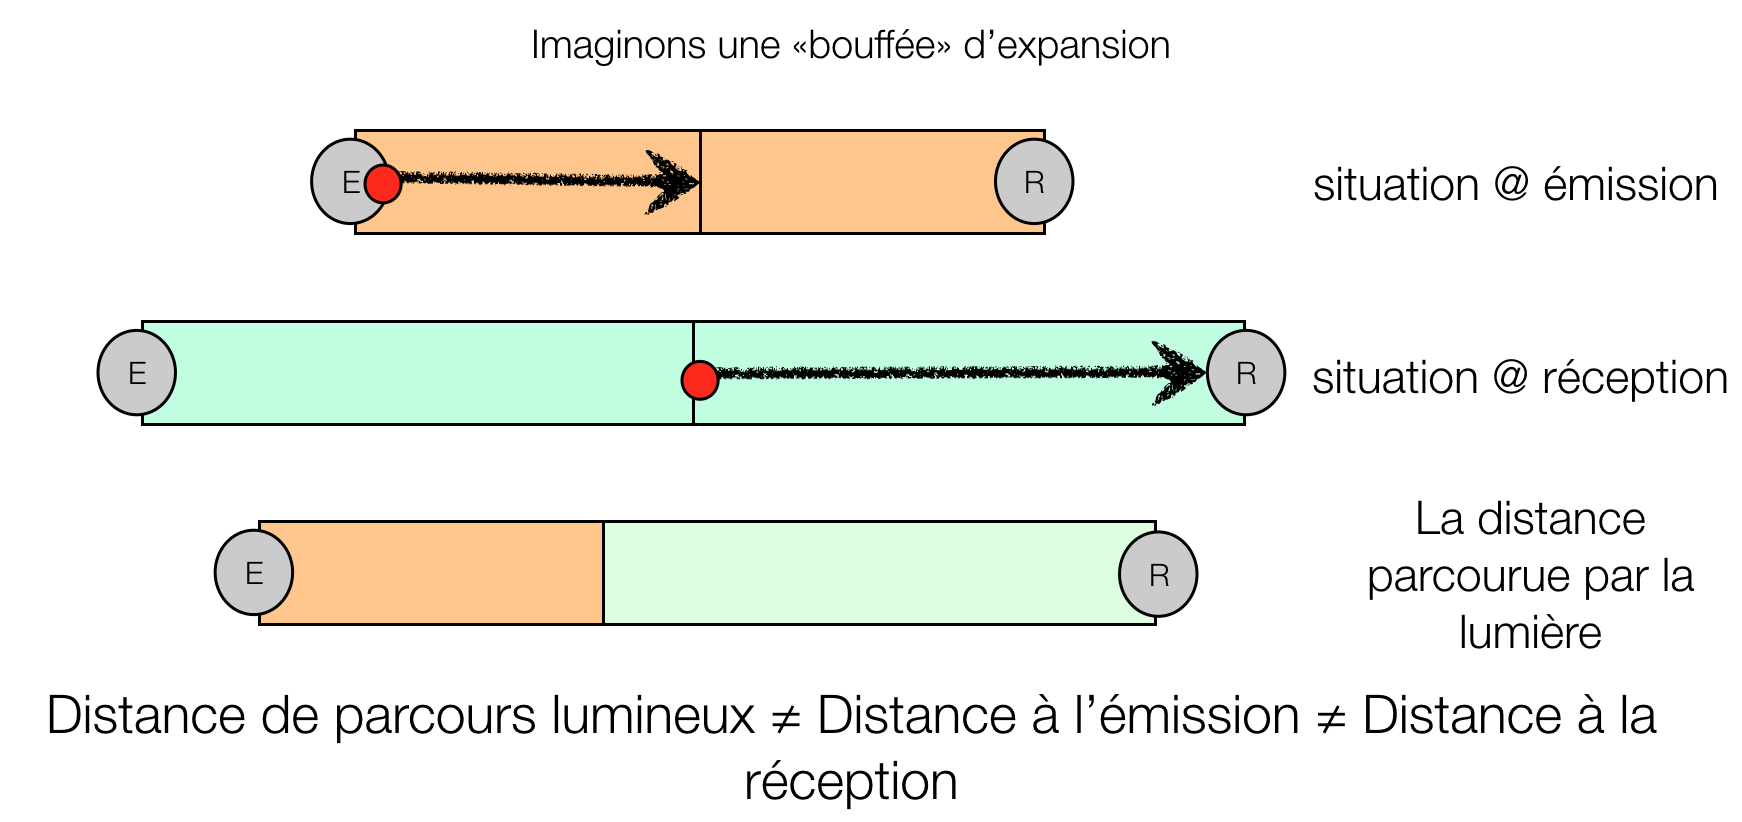
\includegraphics[height=10cm]{figs/dlum.png}
	\caption[Distance de parcours lumineux]{On considère un photon émis en E et reçu en R. Pour simplifier, les distances subissent une expansion instantanée au moment où le photon a parcouru la moitié de la distance initiale entre E et R. 3 distances peuvent être également considérées dans cette expérience de pensée : la distance physique entre E et R \textit{à l'émission} (représentée par 2 blocs courts), la distance physique entre E et R \textit{à la réception} (représentée par 2 blocs longs) et la distance effectivement parcourue par le photon entre l'émission et la réception (représentée par un bloc long et un bloc court). Ces trois distances sont différentes dans un Univers non statique. }
	\label{f:dlum}
\end{figure}

Là où la distance comobile était une quantité statique, la distance physique est une quantité évolutive, dont la dépendance temporelle est encodée par le facteur d'expansion $a(t)$. Notons que si l'on considère le parcours d'un photon\index{photon} sur un intervalle infinitésimal ($t$ est alors quasi constant et $r_0<<1$) alors $dr=cdt$ et la distance physique est celle effectivement parcourue par le rayon lumineux. Considérons à présent un intervalle non-infinitésimal : si la géométrie intrinsèque de l'Univers est plane, nous avons $K=0$ et la distance de parcours lumineux \index{distance de parcours lumineux} \textit{dans ce cas précis} vaut 
\begin{equation}
D_L=\int_{t_e}^{t_r} dr=\int_{t_e}^{t_r}a(t)dr_0,
\end{equation}
où $t_e$ et $t_r$ désignent les instants d'émission et de réception de ce photon sur notre intervalle. Or cette quantité est différente des distances physiques mesurées à l'instant $t_e$ et à l'instant $t_r$:
\begin{eqnarray}
r(t_e)=a(t_e)r_0 &\ne & D_L\\,
r(t_r)=a(t_r)r_0  &\ne & D_L
\end{eqnarray}
car $a(t)$ varie au cours de la trajectoire du photon. On a donc 3 distances différentes (voir aussi la figure \ref{f:dlum}) alors que les extrémités sont identiques dans les 3 cas : ces 3 définitions sont valides mais il faut savoir exactement de quoi il est question \sidenote{en particulier, les articles 'grand public' entretiennent fréquemment cette confusion} ! Par ailleurs, si la courbure de l'espace est positive et non nulle, $K>0$, alors 
\begin{equation}
 D_L>\int_{t_e}^{t_r} a(t)dr_0
\end{equation}
et dans le cas d'une courbure négative, $K<0$
\begin{equation}
D_L<\int_{t_e}^{t_r} a(t)dr_0.
\end{equation}
Cette différence traduit le fait que la lumière voyage en épousant à chaque instant la géométrie de l'espace qu'elle parcourt \sidenote{la lumière parcourt des \textit{géodésiques} de l'espace-temps}, rallongeant ou raccourcissant son trajet par rapport à la distance physique 'brute' des points qu'elle relie. 

De façon générale, la courbure\index{courbure} induit un départ de la distance physique par rapport à une fonction simple de la distance comobile. Considérons à nouveau la distance physique en se plaçant à un instant donné et en calculant $r(t)$ entre 2 points A et B, séparés d'une distance comobile $R_0$ le long d'une direction avec $(\theta,\phi)$ donnés. En pratique il s'agit d'intégrer l'équation \ref{e:phydist} tout en considérant $t$ constant. On a alors
\begin{eqnarray}
&&a(t)R_0\\
r(t)&=&a(t)R_K \arcsin(R_0/R_K)\\
&&a(t)R_K \mathrm{argsh}(R_0/R_K)
\end{eqnarray}
pour une courbure $R_K=K/|K|^{3/2}$ respectivement nulle, positive et négative. Notons que les termes de courbure sont indépendants du temps. Les trois solutions peuvent être résumées sous la forme d'une équation unique $r(t)=a(t)S_K(r_0)$. A nouveau, les distances physiques sont des fonctions du temps qui ne dépendent que de la variation temporelle du facteur d'expansion $a(t)$. Si $a$ est un fonction croissante, \textit{toutes} les distances physiques augmentent avec le temps et on parle d'Univers en expansion\index{expansion}. A l'inverse, $a(t)$ peut être une fonction décroissante du temps dans certains modèles, auquel cas l'Univers est en contraction\index{contraction}.

Pour finir, mentionnons que les distances physiques aujourd'hui sont obtenues en prenant la valeur du facteur d'expansion aujourd'hui. Ces types de quantités mesurées aujourd'hui sont notées par convention avec l'indice 0. Par exemple le temps qui a pu s'écouler depuis le Big-Bang\index{Big-Bang} jusqu'à aujourd'hui est noté $t_0$ : c'est la définition même de l'âge actuel de l'Univers\index{age de l'Univers@âge de l'Univers}. De même le facteur d'expansion aujourd'hui est noté $a_0=a(t_0)$.
\textit{Par convention} le facteur d'expansion est normalisé à cette valeur actuelle et 
\begin{equation}
a_0=a(t_0)=1.
\end{equation}
Il en découle que 
\begin{equation}
r(t_0)=S_K(r_0).
\end{equation}
et dans le cas sans courbure, on constate que la distance physique mesurée aujourd'hui est égale à la distance comobile $r(t_0)=r_0$.

\begin{figure}[htbp]
	\centering
		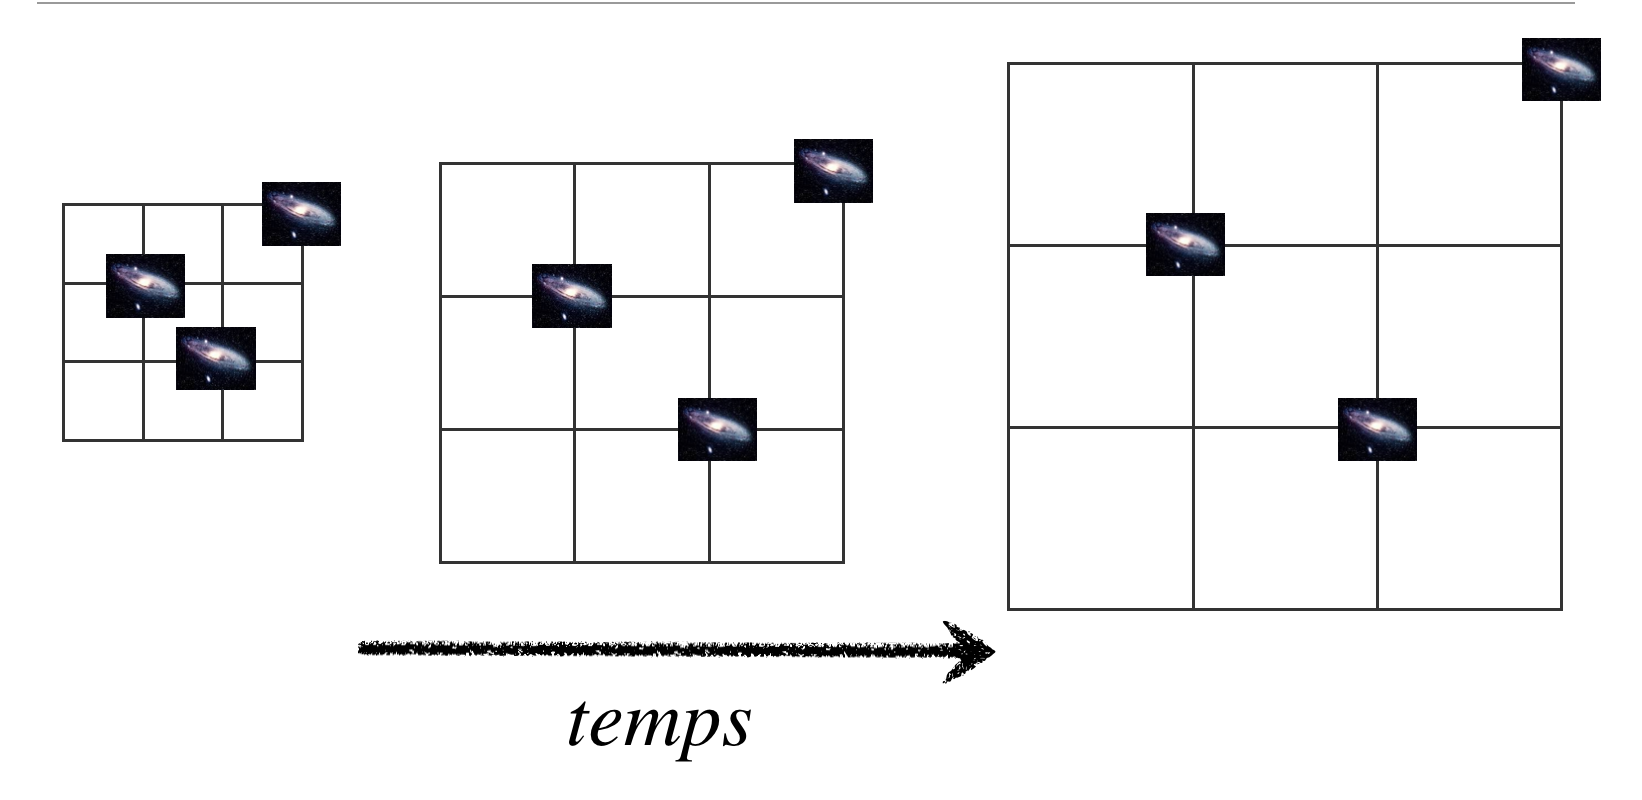
\includegraphics[height=10cm]{figs/grille.png}
	\caption[Coordonnées comobiles et expansion]{Une représentation schématique de la différence entre distance comobile et physique. Ces trois galaxies s'éloignent les unes des autres au cours du temps sous l'effet de l'expansion de l'Univers : l'espace se "dilate" comme indiqué par la grille dont les carreaux deviennent de plus en plus grands. La distance comobile est la distance mesurée en unités de carreaux : ces distances ne varient pas au cours du temps, car les galaxies sont immobiles par rapport à leur espace local. La distance physique, est la vraie distance mesurée avec une règle sur cette page : de façon évidente celle-ci varie pour toutes les paires de galaxies. Notons que ces distances physiques varient mais fondamentalement les galaxies sont toutes immobiles par rapport à l'espace sur lesquelles elles reposent.}
	\label{f:grille}
\end{figure}

\subsection{Facteur d'expansion, Loi de Hubble}
La distance physique $r(t)$ entre deux points peut être simplement dérivée au cours du temps.
\begin{equation}
\dot r(t)= \dot a S_K(r_0) =\frac{\dot a}{a}r(t).
\end{equation}
On définit la \textit{fonction de Hubble}\index{Hubble!fonction} comme la fonction dépendante du temps donnée par :
\begin{equation}
H(t)=\frac{\dot a}{a}.
\label{e:hubble}
\end{equation}
A l'aide de cette nouvelle fonction, le taux de variation des distances peut s'exprimer comme une fonction linéaire de la distance, \textit{la loi de Hubble}\index{Hubble!loi}
\begin{equation}
\dot r(t) = H(t) r(t).
\label{e:hubble2}
\end{equation}
Si $a$ est une fonction croissante, les distances physiques varient d'autant plus qu'elles sont importantes.

Plusieurs remarques peuvent être faites à propos des Eqs \ref{e:hubble} et \ref{e:hubble2}.  La première est que la fonction de Hubble n'est pas une constante temporelle, en revanche sa valeur ne dépend pas du point de l'espace considéré : on peut considérer que c'est une constante \textit{spatiale} de valeur donnée dans tout l'Univers à un instant donné. Suivant la convention générique en cosmologie, sa valeur actuelle est notée avec un indice 0 et vaut environ
\begin{equation}
H_0 \sim 70 \mathrm{km/s/Mpc}.
\end{equation}
Cette valeur est déterminée expérimentalement via par exemple la mesure conjointe des distances et des vitesses de fuites d'objets à grande distance. Cette mesure nécessite une connaissance de la luminosité\index{luminosité} intrinsèque de ces objets \sidenote{on parle aussi de chandelles standards} : par comparaison avec leur luminosité apparente, la distance peut être déduite tandis que la vitesse s'obtient à partir du décalage vers le rouge\index{redshift}. Un diagramme de Hubble\index{Hubble!diagramme} peut alors être construit pour obtenir la valeur de $H_0$ (voir Fig. \ref{f:hubblediag}).
\begin{figure}[htbp]
	\centering
		\includegraphics[height=10cm]{figs/hubble.png}
	\caption[Diagramme de Hubble]{Diagramme de Hubble représentant la vitesse de fuite de différentes sondes astrophysiques à partir des données de Freedman et al. (2000). La ligne trace la relation attendue pour une valeur $H_0=72$ km/s/Mpc tandis que chaque point représente un objet dont la distance et la fuite sont connues. Les objets considérés sont soit des supernovæ (points bleus) soit des galaxies (points orange, vert et rouge) dont les distances sont déterminées avec 3 techniques différentes. On note que les supernovæ permettent de sonder les distances les plus lointaines et sont donc les plus contraignantes pour la mesure du paramètre de Hubble. }
	\label{f:hubblediag}
\end{figure}

On peut constater au vu des unités employées et au vu de la structure de l'équation \ref{e:hubble}, que le paramètre de Hubble a la dimension de l'inverse d'un temps. On définit ainsi le temps de Hubble par $t_H=H^{-1}$~: on verra par la suite que ce temps de Hubble\index{Hubble!temps} est une bonne approximation de l'âge de l'Univers\index{age de l'Univers@âge de l'Univers}. 

La seconde remarque porte sur le caractère linéaire de l'équation \ref{e:hubble2}~: on peut montrer que cela permet de conserver le caractère isotrope et homogène des points de vue (cf. Fig. \ref{f:canard}), comme exigé par le principe cosmologique\index{principe cosmologique}. Si la loi avait été constante ($\dot r \sim r^0$) ou bien quadratique ($\dot r\sim r^2$), l'homogénéité aurait été perdue. 

La dernière remarque porte sur le fait que la loi donnée par l'Eq. \ref{e:hubble2} donne l'impression que des récessions supraluminiques\index{supraluminique} sont autorisées ($\dot r>c$)~: il s'avère que cela est exact, mais le taux de variation de distance calculé ici n'implique pas de déplacement par rapport à un référentiel local inertiel (qui lui serait limité par $c$)\sidenote{ et qui est le régime d'application de la relativité restreinte} mais se rapporte à une dilatation  même de l'espace~: dit rapidement, ceci n'est pas la vitesse d'un corps en déplacement. Par exemple, insistons sur le fait que cette dilatation ne permet pas de transmettre d'information\index{information}.

\begin{figure}[htbp]
	\centering
		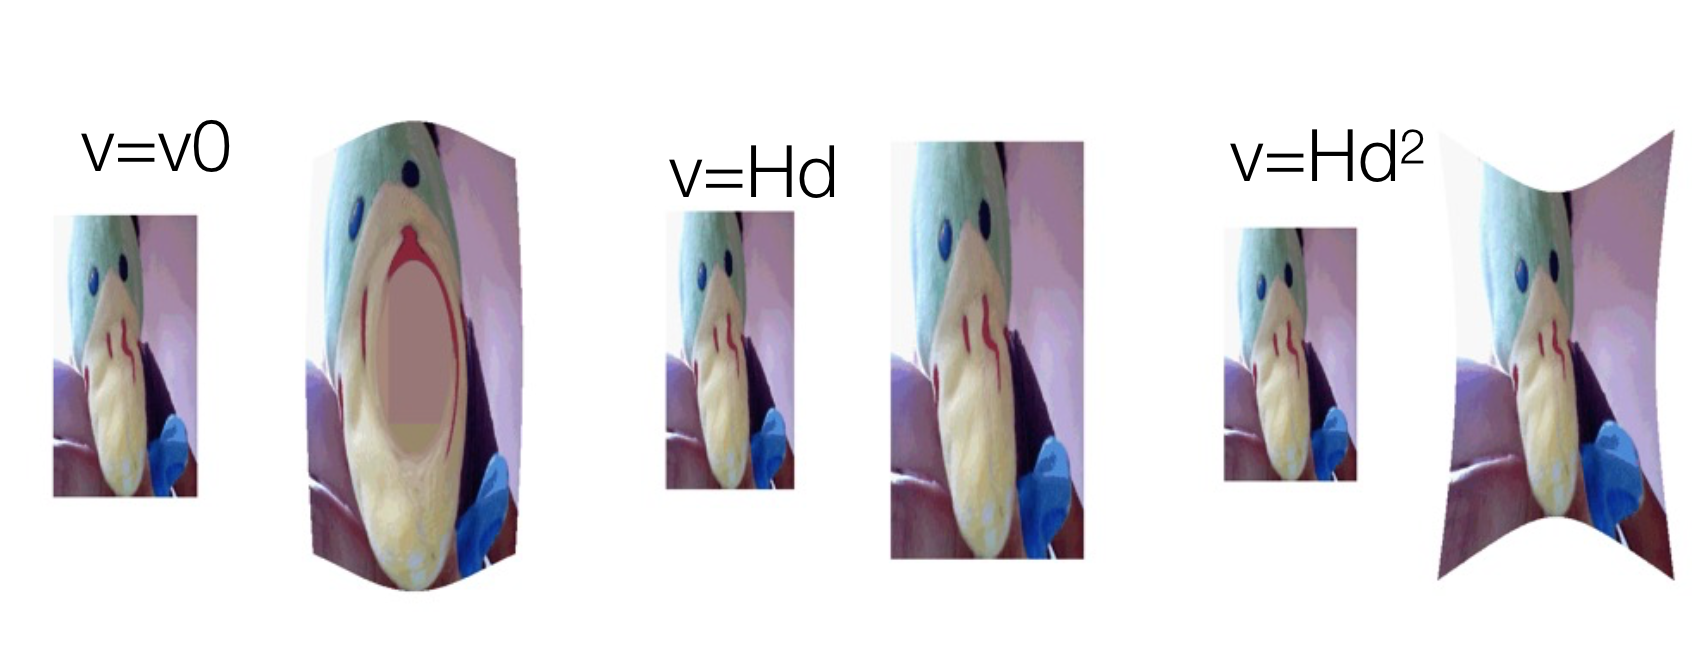
\includegraphics[height=6cm]{figs/canard.png}
	\caption[loi de Hubble et homogénéité]{La loi de Hubble établi une relation linéaire entre vitesse et distance physique. L'image du milieu montre comment une image est déformée par une telle loi linéaire, en fonction de la distance du pixel au centre de l'image : le canard devient plus grand mais n'est en pratique pas déformé. Les deux autres exemples montrent le même type de transformation mais en appliquant une déformation constante en fonction de la distance ou bien une déformation variant comme le carré de la distance. Dans ces 2 cas, le canard est déformé : si ce type de transformation avait été appliquée à un milieu homogène, cette dernière aurait été brisée. Par ailleurs, cette brisure dépendrait du choix de l'origine, en contradiction avec le principe d'homogénéité des points de vues.}
	\label{f:canard}
\end{figure}

\subsection{Décalage vers le rouge}
Nous venons de voir que la forme de la métrique FRW\index{Friedmann-Robertson-Walker!métrique} conduit naturellement à la Loi de Hubble. Dans le même ordre d'idée, la métrique FRW conduit naturellement à une modification de la perception des intervalles temporels. Si l'on considère par exemple l'émission d'un photon\index{photon} depuis un point E jusqu'à sa réception au point R, l'intervalle séparant les deux évènements est nul, $ds^2=0$, comme c'est toujours le cas pour une particule sans masse et se déplaçant à la vitesse de la lumière. Soit $E$ l'origine du système de référence, alors E et R se trouvent sur un seul et même rayon-vecteur ($d\theta=d\phi=0$) et FRW permet d'écrire:
\begin{equation}
\int_{t_E}^{t_R}c\frac{dt}{a(t)}=\int_{r_E}^{r_R}\frac{ dr_0}{\sqrt{1-Kr_0^2}}.
\end{equation}
Considérons un second photon qui va effectuer le même parcours mais en étant émis à l'instant $t_E+\delta_E$ et reçu à l'instant $t_R+\delta_R$. Dans un espace-temps statique, on s'attend à obtenir $\delta_E=\delta_R$. Pour ce second photon FRW permet d'écrire:
\begin{equation}
\int_{t_E+\delta_E}^{t_R+\delta_R}c\frac{dt}{a(t)}=\int_{r_E}^{r_R}\frac{ dr_0}{\sqrt{1-Kr_0^2}}.
\end{equation}
Notons que les bornes d'intégration du second membre restent inchangées, le second photon passant par les 2 même endroits en coordonnées comobiles: par conséquent les 2 intégrales temporelles des 2 photons sont identiques permettent d'écrire la relation :
\begin{equation}
\int_{t_E}^{t_E+\delta_E}c\frac{dt}{a(t)}=\int_{t_R}^{t_R+\delta_R}c\frac{dt}{a(t)}.
\end{equation}
Si l'on suppose que les délais temporels\index{délais temporels} $\delta_E$ et $\delta_R$ sont suffisamment petits par rapport au temps typique d'évolution du facteur d'expansion $a$, alors l'on obtient que le délai mesuré à la réception diffère du délai à l'émission:
\begin{equation}
\delta_R=\frac{a(t_R)}{a(t_E)} \delta_E.
\end{equation}
Cette relation est valable pour tous les délais~: si la métrique n'est pas statique $a(t_E)\neq a(t_R)$, les délais sont modifiés. Par exemple on constate que les courbes de lumières de supernovæ\index{supernovæ} sont affectées par cette modification des délais (voir Fig. \ref{f:wSN}). De même les flux\index{flux} de photons\sidenote{flux qui sont des nombres de photons reçus par intervalle de temps} subissent une "dilution" cosmologique à cause d'une modification de la durée s'écoulant entre 2 photons successifs. Enfin la \textit{longueur d'onde} $\lambda=cT$ est directement proportionnelle à une durée (la période). La longueur d'onde\index{longueur d'onde} d'un rayonnement électromagnétique reçu aujourd'hui est donc aussi affectée~:
\begin{equation}
\lambda_0=\frac{\lambda_E}{a(t_E)}
\end{equation}
où on a utilisé la convention $a(t_0)=1$. Il en découle que le décalage vers le rouge\index{redshift} est donné par
\begin{equation}
z = \frac{\lambda_0-\lambda_E}{\lambda_E}=\frac{1}{a_E}-1.
\end{equation}
Si le facteur d'expansion était plus petit dans le passé (comme attendu pour un Univers en expansion), le décalage vers le rouge (ou \textit{redshift}) est positif ou nul. Notons qu'à aucun moment il n'est fait mention de vitesse de déplacement de source ou de récepteur. Le seul effet est celui d'un espace-temps non-statique qui donne un effet similaire à un effet Doppler mais qui en aucun cas ne nécessite que la source ou l'émetteur possèdent une vitesse non-nulle par rapport à son référentiel localement inertiel.

\begin{figure}[htbp]
	\centering
		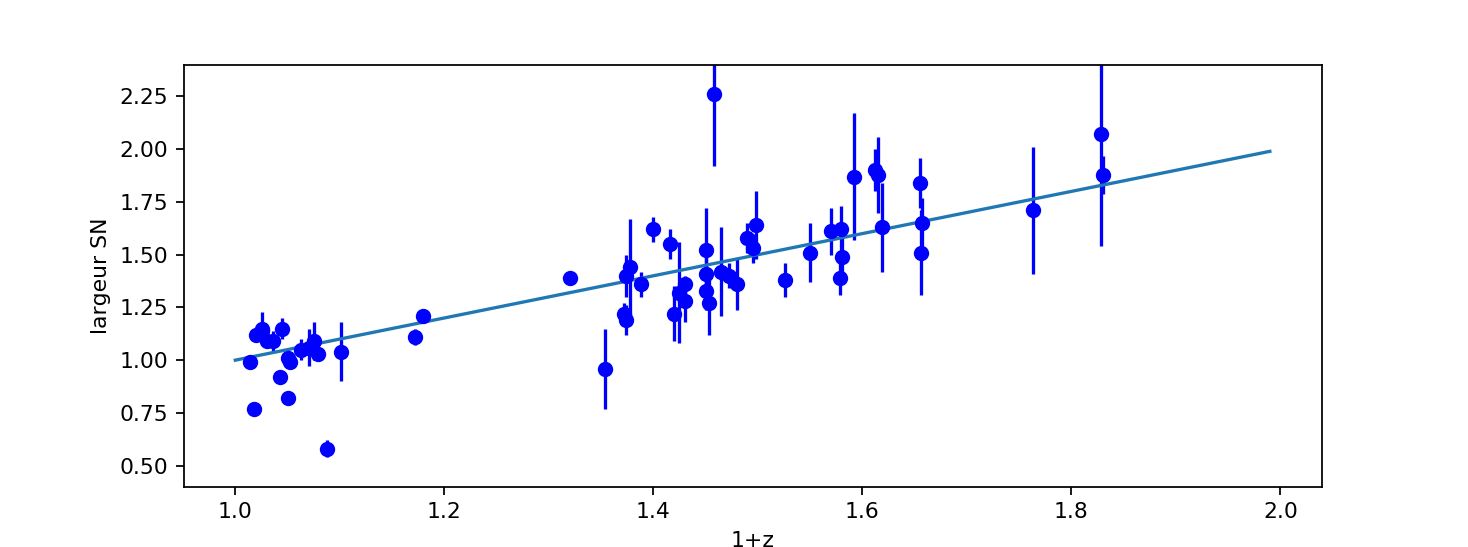
\includegraphics[height=6cm]{figs/wSN.png}
	\caption[Durée des supernovæ en fonction du redshift]{Un exemple de mesure des durées des supernovæ cosmologiques en fonction du redshift. Tous ces objets ont des courbes de lumières identiques car correspondant à l'explosion d'objets très similaires (des naines blanches d'environ 1.4 $M_\odot$). On constate que la durée des courbes de lumières associées varient en suivant une loi en $1+z$ où $z$ est le redshift : c'est l'effet cosmologique de dilatation des durées qui opère ici. Données issues de Goldhaber et al. 2001.}
	\label{f:wSN}
\end{figure}

\subsection{Source de la gravitation}
A ce stade, l'élément essentiel qui reste à préciser est la loi qui régit l'évolution du facteur d'expansion et par extension celle de la métrique FRW\index{Friedmann-Robertson-Walker!métrique}. Plus généralement quelles sont les lois qui permettent de relier la métrique $g_{\mu\nu}$ (donc la structure de l'espace-temps) aux sources de la gravitation ? Ces relations sont connues et portent le nom d'équations d'Einstein\index{equation d'Einstein@équation d'Einstein}. Leur détermination exacte est une démarche relativement complexe mais le cheminement logique qui aboutit à leur obtention peut être aisément décrit. 

Un bon point de départ est l'équation de champ de la gravitation Newtonienne, à savoir l'équation de Poisson\index{equation de Poisson@équation de Poisson}. Elle relie la densité de matière $\rho$ au potentiel gravitationnel\index{potentiel gravitationnel} $\phi(x)$, qui est une fonction simple du champ de gravitation~:
\begin{equation}
\Delta \phi =\rho.
\label{e:poisson}
\end{equation}
Clairement, le potentiel gravitationnel a pour source la densité de matière. En RG, l'objectif est d'obtenir une équation de champ analogue mais reliant $g_{\mu\nu}$ à ses sources. Disons d'emblée que dans le régime des champs faibles( dans lequel la gravitation Newtonienne s'applique) métrique et potentiel gravitationnel sont directement relié.

Quelles sont à priori les sources de la métrique en RG ? Une première tentative peut être effectuée en considérant directement la densité de matière \index{densité!matière}$\rho$ comme source~: c'est le cas quand les champs sont faibles et la matière est source de gravitation donc de géométrie. Toutefois on sait également que la masse en tant que telle ne joue pas de rôle central dans les théories relativistes, c'est davantage \textit{l'énergie}\index{energie@énergie} $E$ qui joue un rôle de premier plan. 

La \textit{densité} énergie serait-elle cette source ? Il est clair qu'elle doive jouer un rôle, par exemple au travers de la densité d'énergie de masse $\rho c^2$, ce qui reviendrait simplement à considérer la contrepartie énergie de la source de gravité Newtonienne. La difficulté de cette option réside dans le fait que l'énergie n'est pas directement une quantité fondamentale, y compris en relativité restreinte~: l'énergie n'est qu'une composante d'un concept plus vaste qui est l'énergie-impulsion \sidenote{par ailleurs la valeurs de l'énergie dépend du système de référence choisi, ce qui plaide en sa défaveur}. Par conséquent si l'énergie source la gravité en RG, c'est au travers de l'énergie-impulsion\index{energie@énergie!énergie-impulsion} et non seule. Plus précisément c'est au travers d'une \textit{densité} d'énergie-impulsion.

Si on note l'énergie impulsion $(P^0,P^1,P^2,P^3)$ où $P^0=E$ (en supposant $c=1$), on arrive à des expressions de densités de type:
\begin{equation}
\frac{dP^\mu}{dx^\alpha dx^\beta dx^\gamma}.
\end{equation}
Notons que $\alpha,\beta,\gamma$ désigne toutes les coordonnées disponibles, \textit{temps} compris. Bien sûr la densité d'énergie sus-mentionnée fait partie des sources:
\begin{equation}
\frac{dE}{dx dy dz},
\end{equation}
tandis que l'expression suivante est tout aussi légitime pour constituer un terme source de la gravité:
\begin{equation}
\frac{dP_x}{dtdydz}.
\end{equation}
Cette dernière expression désigne une force ($dP_x/dt$) divisée par une surface $dydz$ à $x$ constant\sidenote{c'est littéralement le flux de $P$ par unité de temps au travers de la surface $dydz$ perpendiculaire à $dx$}, à savoir une pression suivant la direction $x$\index{pression}. Notons qu'une pression est homogène à une densité d'énergie.

En généralisant cette expression, on obtient le tenseur des contraintes ou \textit{tenseur énergie-impulsion}
\begin{equation}
T^{\mu\delta} = \frac{dP_\mu}{dx^\alpha dx^\beta dx^\gamma}.
\end{equation}
obtenu en considérant la densité de la composante $\mu$ de $P$ sur la "surface" de coordonnées $x^\delta$ constante. C'est la source de la métrique, qui généralise la densité de masse du cas newtonien.  Comme mentionné ci-dessus, la densité d'énergie a donc un rôle à jouer mais également la pression, de même que le cisaillement \sidenote{qui est une force parallèle à une surface, complémentaire à la pression qui est perpendiculaire à une surface}. Par la suite la contribution d'un type d'énergie à la dynamique de l'espace-temps devra s'évaluer au vu de toutes ces quantités. 

Notons que $T$ obéit à une équation analogue à généralisation de la conservation de l'énergie\index{conservation de l'énergie} dans un espace-temps quelconque : 
 \begin{equation}
 \nabla_\nu T^{\mu\nu}=0,
 \label{e:divT}
 \end{equation}
 cette relation est tensorielle et non triviale et définit une "conservation" globale de l'objet $T$. La densité d'énergie est l'une des composantes de cet objet et n'est pas généralement conservé \textit{individuellement}, ne serait-ce que parce que l'expression de la densité d'énergie dépend du système de coordonnées choisi.

A ce stade, le terme source de la dynamique de l'espace-temps est connu, reste à expliciter l'opérateur différentiel qui agit sur la métrique et qui joue un rôle analogue au laplacien de l'équation \ref{e:poisson}. En d'autres termes quel est le tenseur $G$ , fonction de la métrique qui permette d'avoir:
\begin{equation}
G^{\mu\nu}=T^{\mu\nu}.
\end{equation}
Sans rentrer dans les détails, on cherchera à obtenir un opérateur différentiel du second ordre, tout comme pour l'équation de Poisson\index{equation de Poisson@équationde Poisson} newtonienne. De plus il faut que l'équation \ref{e:divT} soit satisfaite par $G$. L'opérateur différentiel du second ordre le plus simple permettant de satisfaire à cette contrainte est le \textit{tenseur d'Einstein}\index{tenseur d'Einstein}
\begin{equation}
G^{\mu\nu}=R^{\mu\nu}-\frac{R}{2}g^{\mu\nu}
\label{e:einstein}
\end{equation}
où $R^{\mu\nu}$ est le tenseur de Ricci\index{tenseur de Ricci} ou \textit{tenseur de courbure} et qui dépend de dérivées de second ordre de $g^{\mu\nu}$. $R$ est la trace de ce tenseur et est appelé aussi scalaire de courbure ou scalaire de Ricci.

Pour résumer, l'équation de champ de la gravité dans le cadre de la relativité générale décrit le comportement de la métrique en fonction du contenu local en énergie, via :
\begin{equation}
G^{\mu\nu}=T^{\mu\nu}.
\label{e:RG}
\end{equation}
Plusieurs remarques peuvent être faites à ce stade. La première est que nous sommes passé d'une équation scalaire dans le cas newtonien à une équation tensorielle avec dans l'absolu $ 4\times 4=16$ équations couplées à résoudre. Toutefois le tenseur d'énergie-impulsion\index{energie@énergie-impulsion} est symétrique et au final seules 10 équations restent réellement indépendantes dans le cas générique. De plus si les sources d'énergies possèdent un certain degré d'isotropie (comportement de fluide parfait\index{fluide parfait}\sidenote{c'est-à-dire un fluide sans viscosité ni cisaillement} par exemple) les composantes anisotropes de la pression ne rentrent pas en jeu et le système peut encore être réduit. La seconde remarque porte sur la structure du tenseur d'Einstein (Eq. \ref{e:einstein}). On constate ainsi que l'opérateur est non linéaire  en métrique (via par exemple $\frac{R}{2}g^{\mu\nu}$), ce qui rend l'équation de champ particulièrement complexe à résoudre dans le cas général. On constate également que la métrique $g^{\mu\nu}$ est elle-même source de courbure. Cela est particulièrement manifeste en écrivant l'équation \ref{e:RG} avec un terme supplémentaire:
\begin{equation}
G^{\mu\nu}=T^{\mu\nu}+\Lambda g^{\mu\nu}
\label{e:modifeins}
\end{equation}
où $\Lambda$ est un scalaire constant dans l'espace-temps. Compte tenu de $\nabla_\mu g^{\mu \nu}=0$, il en découle que l'équation \ref{e:modifeins} reste valable et dans ce cas  la métrique est également source de courbure. Notons que le scalaire $\Lambda$ introduit dans l'équation Eq. \ref{e:modifeins} s'interprète comme une \textit{constante cosmologique}\index{constante cosmologique}.

\section{Équations de Friedmann}
Comme indiqué dans la section précédente, l'hypothèse d'un Univers homogène et isotrope conduit à une forme de la métrique donnée par FRW\index{Friedmann-Robertson-Walker!métrique}. Considérant de plus que la relativité générale fournit une bonne description de la dynamique de l'espace temps, on est en principe capable de résoudre les équations d'Einstein pour une métrique FRW. Le résultat de cette opération est \textit{l'équation de Friedmann}. Elle repose sur la RG, sur la métrique de FRW et considère que le contenu en énergie de l'Univers est bien décrit par des "fluide" parfaits\index{fluide parfait}, de pression isotrope et sans viscosité.

L'équation de Friedmann\index{equation de Friedmann@équation de Friedmann} est une relation scalaire qui relie le facteur d'expansion $a(t)$, qui restait la dernière quantité non précisée de la métrique, au contenu en énergie de l'Univers~:
\begin{equation}
\frac{\ddot a}{a}=-\frac{4\pi G}{3c^2}(\rho c^2 +3 P),
\label{e:friedmann}
\end{equation}
où $\rho c^2$ est la densité d'énergie de l'Univers et $P$ sa pression, qui sont toutes deux fonctions du temps et donc de $a$. On constate que comme prévu, la dynamique de l'espace temps est lié à son contenu énergétique. Notons que \textit{à priori} le second terme est défini positif, donc la dynamique de l'Univers semble être décélérée $\ddot a<0$. Un modèle d'Univers se définira à partir d'une solution de cette équation différentielle, qui elle même dépendra du contenu en énergie. C'est l'objet du chapitre suivant.